\chapter{Introduction}

\vspace{10mm}

\begin{quote}
  {\it   
  ``Jam sessions, jitterbugs and cannibalistic rhythmic orgies are
  wooing our youth along the primrose path to Hell!''} --- The Most
  Reverend Francis J.L. Beckman in an address to the National Council
  of Catholic Women, Biloxi, Mississippi, October 25, 1938
\end{quote}

\begin{quote}
  {\it   
    ``Without music, life would be a mistake... I would only believe in a
  God that knew how to dance.''} --- Friedrich Nietzsche
\end{quote}


\vspace{7mm}
\section{Some Personal Compositional Perspectives on Rhythm}
\vspace{5mm}


My interest in understanding rhythm comes from my struggles 
to write music that incorporates rhythm in fresh 
and exciting new ways.  Frequently while listening, 
I am deluged with musical ideas for a new work or work 
already in progress.  Many times, I find it difficult 
to pick out the individual patterns or understand, in real 
time, how different components of a percussion mix interrelate.  
For the experienced listener and musician this might be a 
routine task, but I would argue that such transparency is 
less common in electronic or dance styles that play with the 
human perceptual limits (Aphex Twin, Squarepusher, etc) especially 
where the recording is the only source of information about the 
underlying musical and rhythmic structure. 


On one hand, repeated listenings and intensive study would facilitate 
a better understanding; however, for the compositional 
novice, a tool that embodied the skills of ear-training and expert 
knowledge on rhythm perception that could uncover the hidden 
structure and more complex inter-relationships between various 
elements of a mix, would be invaluable. 

Another compositional use of such a tool would be to aid mapping out 
new rhythmic configurations in a more orderly fashion.  Rather than 
employing music theoretic heuristics with ad-hoc trial and error 
experiments, new patterns could be systematically found by traversing 
{\it Rhythmic Spaces}, (defined below). The problem with trial and error 
is that it is time consuming. Managing the complexity of the
interrelationships between patterns and where they reside in the 
rhythmic space becomes unwieldy as the said patterns accumulate. With a 
computational tool, such an effort would be markedly simpler 
especially if rhythmic features are modeled parametrically. 
Several features that might be interesting to explore are 
onset timing intervals, accentuation of onsets, overall tempo 
and timing and grouping hierarchies between elements of a mix. 
A ``rhythmic space traversal'' would take a rhythmic pattern 
with certain of the above features and hold all but one constant 
while creating new patterns that varied the last feature in some way.

\begin{figure}[thp]
  \begin{center}
    \resizebox{3.5in}{!}{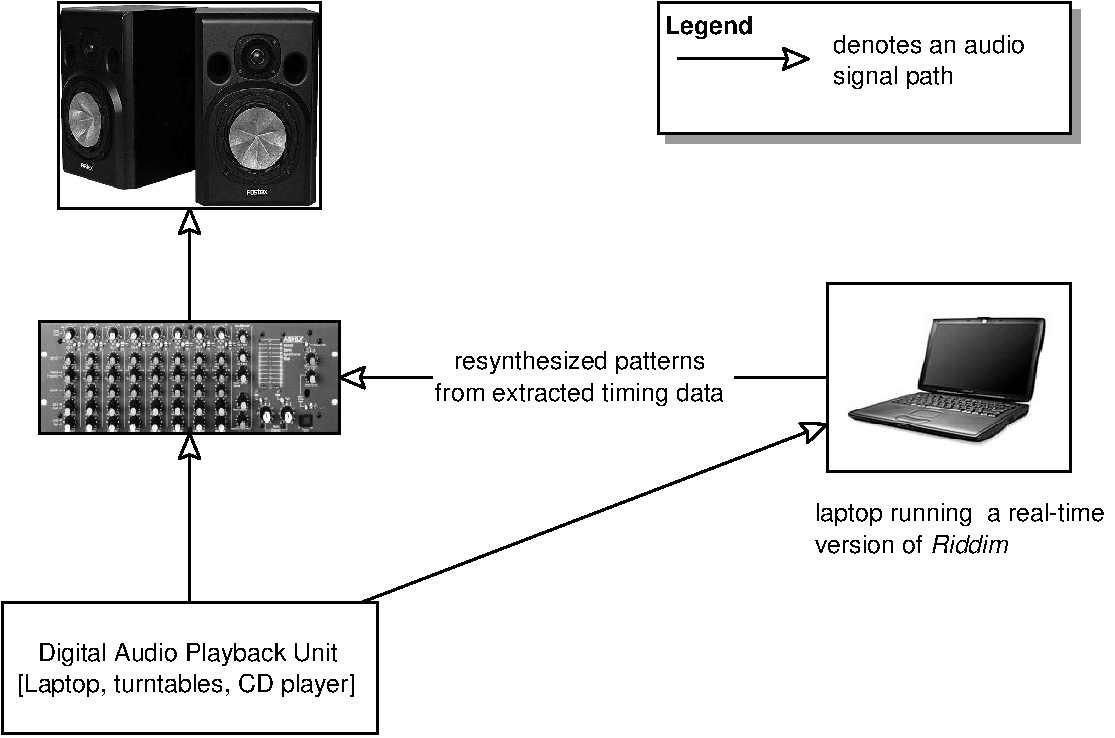
\includegraphics{realtimeRiddim.pdf}}
    \caption{Live performance with Riddim}
    \label{A real-time possibility of Riddim} 
  \end{center}
\end{figure}

\vspace{7mm}
\section{Towards a General Perceptual, Transcriptive Computational Tool}
\vspace{3mm}

A perceptual {\sl and} transcriptive tool is most useful to meet the 
compositional objectives described above.  It needs to be
transcriptive because resynthesis can only take place from an abstract
representation. It also needs to be perceptual because no score or
advanced knowledge about the structure of the music may be available.
In this case, any structure the listener perceives is inferred
via direct perception.  This is especially true of many styles,
especially ones practiced solely in oral traditions. 
Is everything that is needed for a perceptual transcriptive
representation of rhythm present in the recorded audio?  The
information {\sl must} be contained in the structure of the audio
waveform because it is this same audio that is processed 
and understood by the brain. 

In the past, researchers have tended to focus on a very specific area 
of rhythm, be that tempo, beat-induction, metrical interpretation or 
rhythmic pattern recognition. Only rarely did they ever integrate 
their work in a framework concerned with the greater experience of 
rhythm perception.  What is attempted here is the development of a 
tool that explores a more integrative approach. Integrative is used 
in the sense that the streams of timing sequences extracted from an audio 
file can be incorporated in existing interpretive models of rhythm, 
that together can approach a computational correlate of a ``rhythmic percept''.

\vspace{7mm}
\section{Thesis Structure}
\vspace{3mm}

This thesis is structured in the following way. First, I will review the
most salient literature on rhythm, by going through its various dimensions, 
discussing the history and varying opinions. Next I shall discuss my 
approach to developing {\it Riddim}, a rhythm analysis tool designed 
to attempt to meet some of the compositional needs described above.  
This will include some high level algorithmic descriptions of my approach, 
a brief description of the development platform and how the various 
components operate.  Next, I will explain the workings of each of the 
algorithms and illustrate why they are important and how they are 
used, providing detailed diagrams of how data flows through each module.

Finally, I shall show my results which are in-depth rhythmic analyses 
of a variety of musical recordings using {\it Riddim}. {\it Riddim} will
be distributed as a stand alone software application from which commands to
perform a variety of rhythmic analyses can be executed. Results can then
be viewed and saved as MIDI files or rendered as digital audio for use
in subsequent creative settings. 
